\documentclass{ximera}

\input{../../preamble.tex}

\author{Kenneth Berglund}
\acknowledgement{https://www.stitz-zeager.com/szca07042013.pdf}

\begin{document}
\begin{exercise}

You are on a boat on a lake sailing directly towards a lighthouse whose observation deck is 50 feet above the surface of the lake. You spot someone on the lighthouse observation deck and measure the angle of elevation (the angle you have to look up to see the person). Some time later, you measure the angle of elevation again. The first sighting had an angle of elevation of $\pi/6$, and the second sighting had an angle of elevation of $\pi/4$. We want to find out how far your boat has traveled between sightings. 
\begin{enumerate}
%\item What is the angle with your windowsill in radians? $\answer{\frac{5\pi}{12}}$ \\ 
%The angle between Sally's windowsill and her building (in radians)? $\answer{\frac{\pi}{12}}$

\item
First, consider a picture of the problem with all known distances and angles labeled.

		\begin{image}[2in]
		  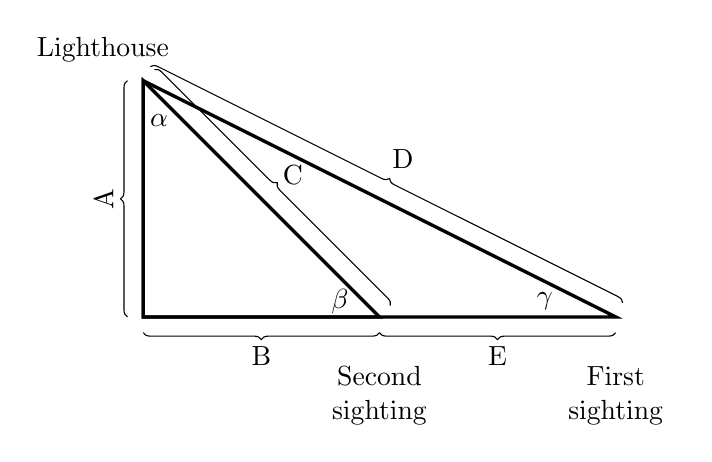
\begin{tikzpicture}
		    \coordinate (C) at (0,2);
		    \coordinate (D) at (0,-1);
		    \coordinate (E) at (3,-1);
			\coordinate (F) at (6, -1);    
		%\tkzMarkRightAngle(C,D,E)
		    %\tkzMarkAngle(C,E,D)
		    %\tkzMarkAngle(D,C,E)
		    \draw[decoration={brace,mirror, raise=.2cm},decorate,thin] (0,-1)--(3,-1);
		    \draw[decoration={brace,mirror,raise=.2cm},decorate,thin] (0,2)--(0,-1);
		    \draw[decoration={brace, raise=.2cm},decorate,thin] (0,2)--(3,-1);
		\draw[decoration={brace, raise=.2cm},decorate,thin] (0,2)--(6,-1);
		\draw[decoration={brace, mirror, raise=.2cm},decorate,thin] (3,-1)--(6,-1);
		    \draw[very thick] (D)--(E)--(C)--cycle;
		\draw[very thick] (D)--(F)--(C)--cycle;    
		\node at (1.5,.-1-.5) {B};
		\node at (4.5,.-1-.5) {E};
		    \node[rotate=90] at (0-.5,.5) {A};
		    \node at (1.9,.8) {C};
		\node at (3.3,1) {D};    
		\node at (.2,1.5) {$\alpha$};
		      \node at (2.5,-.8) {$\beta$};
			\node at (5.1,-.8) {$\gamma$};
		      \node at (-.6,2.4) {\parbox{1.5cm}{\centering Lighthouse}};
		      \node at (3,-2) {\parbox{1.5cm}{\centering Second \\ sighting}};
		      \node at (6,-2) {\parbox{1.5cm}{\centering First \\ sighting}};
		  \end{tikzpicture}
		\end{image}

Label all known lengths and angles with units (exact answers in ft and radians):
\begin{enumerate}
\item $A$ is the \wordChoice{\choice[correct]{\text{height of the lighthouse}}\choice{\text{distance the boat has traveled}}}, which is $\answer{50}$ ft. 

\item $E$ is the \wordChoice{\choice{\text{height of the lighthouse}}\choice[correct]{\text{distance the boat has traveled}}}, which we do not know yet.

\item $\beta$ is the angle of elevation on the \wordChoice{\choice{\text{first}}\choice[correct]{\text{second}}} sighting. \smallskip\\
$\beta = \answer{\frac{\pi}{4}}$ radians.

\item $\gamma$ is the angle of elevation on the \wordChoice{\choice[correct]{\text{first}}\choice{\text{second}}} sighting. \smallskip\\
$\gamma = \answer{\frac{\pi}{6}}$ radians.
\end{enumerate}

\item How far from the lighthouse is the boat at the second sighting? $B = \answer{50}$ ft.

\item How far from the lighthouse is the boat at the first sighting? $B + E = \answer{50\sqrt{3}}$ ft.

\item How far did the boat travel between the two sightings? $E = \answer{50(\sqrt{3} - 1)}$ ft.

\end{enumerate}

\end{exercise}
\end{document}
